\documentclass[10pt]{beamer}


\usepackage[utf8]{inputenc}
\usepackage[brazil]{babel}
\usepackage{graphicx}		% utilizado para inserir gráfico

\usepackage{verbatim}      % Para comentario em bloco

% Usado para incluir código
\usepackage{listings}
% Needed to use citations.
\usepackage{cite}

\usetheme{Copenhagen}
\usecolortheme{lccv}
\setbeamertemplate{background}{
\includegraphics[width=\paperwidth]{./figuras/background_lccv.jpg}}
%\setbeamercovered{transparent}

\title[]{eXtreme Programming}
\author[]{Baltazar Tavares Vanderlei\\
Dielson Sales de Carvalho\\
Priscylla Silva\\
Vinícius dos Santos Oliveira}
%\date{\today}
\institute[2013]{Instituto de Computação - IC/UFAL}

\begin{document}

\begin{comment}
TODO:
Papeis, não tem referencias e não explica quais
Remover parte do meio
Trocar ordem do começo? Principios e valores primeiro e exemplo top-down depois?
Revisar parte de principios, colocar figuras e desenvolver mais
Desenvolver a parte de valores? Falta figuras...
Referencias ... Como fazer ....
\end{comment}

\newcommand{\til}{\~{}}

\frame{\titlepage}
\begin{frame}[t]
  \frametitle{Sumário}
  \tableofcontents[framebreaks]
  % \tableofcontents[pausesections]
\end{frame}

% Perfumaria sobre o sumário ser mostrado a cada passagem de sessão e sub-sessão.
\AtBeginSection[]{
  \begin{frame}[t]
    \frametitle{Sumário}
    \tableofcontents[currentsection]
  \end{frame}
}

\AtBeginSubsection[]{
  \begin{frame}[t]
    \frametitle{Sumário}
    \tableofcontents[currentsubsection]
  \end{frame}
}


%%%%%%%%%%%%%%%%%%%%%%%%%%%%%%%%%%%%%%%%%%%%%%%%%%%%%%%%%%%%%%%%%
\section{XP (eXtreme Programming)}

\subsection{Visão geral}

\begin{frame}
  \frametitle{Visão geral quanto ao tempo}
  \begin{figure}
    \centering
    \makebox[\textwidth]{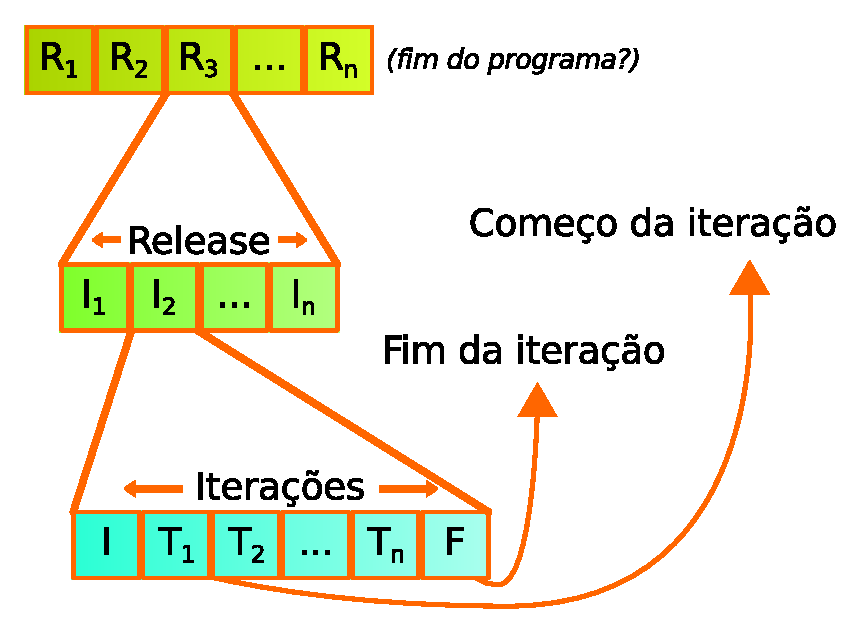
\includegraphics[width=\textwidth]{./figuras/visao_geral_tempo.pdf}}
  \end{figure}
\end{frame}


\begin{frame}
  \frametitle{Visão geral}
  \begin{itemize}%[<+->]
  \item \textbf{Releases}
    \begin{block}{}
      \textbf{Levam meses}, são compostas de \textbf{iterações}
    \end{block}
  \item \textbf{Iterações}
    \begin{block}{}
      São periodos de poucas semanas(tipicamente, de \textbf{1 a 4 semanas}), são compostas de \textbf{tarefas}
    \end{block}
  \item \textbf{Tarefas}
    \begin{block}{}
      São \textbf{atividades basicas}, devem durar idealmente \textbf{1 dia de trabalho}, mas normalmente duram mais.
    \end{block}
  \end{itemize}
\end{frame}


\subsection{Releases}

\begin{frame}
%  \frametitle{Releases}
  \begin{figure}
    \centering
    \makebox[\textwidth]{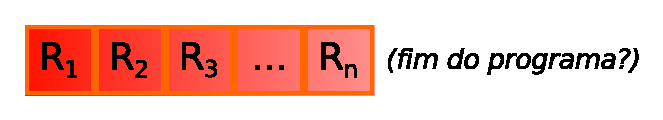
\includegraphics[width=\textwidth]{./figuras/ciclo_release.pdf}}
  \end{figure}
  \begin{itemize}%[<+->]
    \item \textbf{Refletir} sobre o problemas, \textbf{identificar} e/ou \textbf{propor soluções}
    \item \textbf{Cliente} e \textbf{equipe} se reúnem para definir os temas
    \item Cliente controla o \textbf{escopo}, decidindo o que \textbf{fazer} ou \textbf{adiar}
    \item Normalmente, \textbf{3 meses}
  \end{itemize}
\end{frame}

\subsection{Iterações}

\begin{frame}
%  \frametitle{Iterações}
  \begin{itemize}%[<+->]
    \item Incremento \textbf{projetado}, \textbf{programado}, \textbf{testado} e \textbf{entregue}
    \item Ponto de \textbf{avaliação}, \textbf{re-avaliação}, \textbf{feedback}, interação com a \textbf{satisfação do cliente} e \textbf{mudanças}
    \item Esse codigo vai ser \textbf{aprimorado} nas proximas iterações, mas é \textbf{codigo funcional}
    \item No inicio, \textbf{Jogo do planejamento}
    \item No final, o cliente tem a oportunidade de \textbf{utilizar} e \textbf{avaliar} o que foi produzido
    \item Normalmente, \textbf{1 semana}
  \end{itemize}
\end{frame}

\begin{frame}
  \begin{figure}
    \centering
    \makebox[\textwidth]{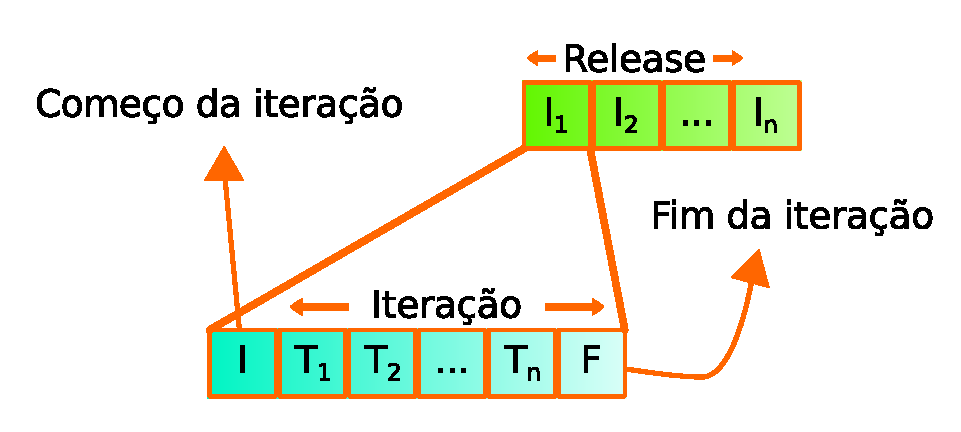
\includegraphics[width=\paperwidth]{./figuras/ciclo_iteracoes.pdf}}
  \end{figure}
\end{frame}

\begin{frame}
  \frametitle{Jogo do planejamento}
    \begin{block}{O cliente}
      \begin{itemize}%[<+->]
        \item Define as histórias(\textbf{User Story})
        \item Decide qual o \textbf{valor de negócio} de cada história
        \item Decide que histórias serão construídas no release
      \end{itemize}
    \end{block}
    \pause
    \begin{block}{Os programadores}
      \begin{itemize}%[<+->]
        \item Estimam \textbf{quanto tempo} será necessário para construir cada história, com base em \textbf{experiencias passadas}
        \item Advertem o cliente sobre \textbf{riscos técnicos significativos}
        \item Medem o \textbf{progresso da equipe} para fornecer um orçamento geral para o cliente
      \end{itemize}
    \end{block}
\end{frame}


\begin{frame}
  \frametitle{Final da Iteração}
  \begin{itemize}%[<+->]
    \item Testes de aceitação
    \item Entrega de \textbf{software para o cliente}
    \item \textbf{Cliente} tem oportunidade de \textbf{testar} e \textbf{avaliar}
  \end{itemize}
  \begin{block}{}
Com base nos resultados, reúne-se novamente com a equipe e estabelece novas prioridades de acordo com o que acabou de aprender com o software e com aquilo que já imaginava ser necessário produzir ao longo do restante do projeto.
  \end{block}
\end{frame}



\subsection{Tarefas}
\begin{frame}
  \begin{itemize}
  \item Compomente basico
  \item É a implementação de uma \textbf{User story} pelo \textbf{par de programadores}
  \item Testes!
  \item Executada de acordo com os \textbf{valores} e \textbf{Práticas do XP}
  \end{itemize}
  \begin{figure}
    \centering
    \makebox[\textwidth]{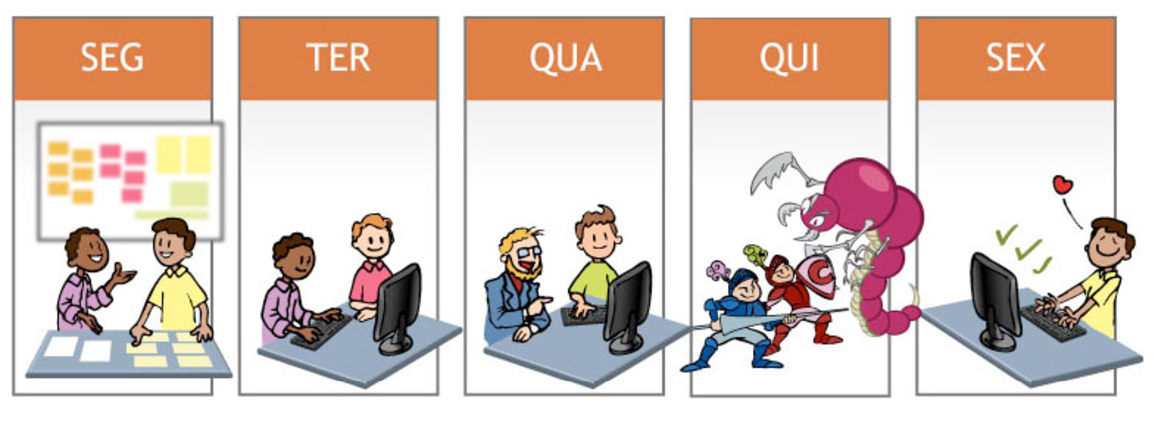
\includegraphics[width=\textwidth]{./figuras/ciclo_geral_tarefas.pdf}}
  \end{figure}
\end{frame}



\subsection{Valores}
\begin{frame}
%  \frametitle{Valores}
  \begin{block}{}
    São o conjunto de valores que a equipe deve seguir, praticar e se comportar em grupo para usar o XP.
  \end{block}
  \begin{itemize}
  \item Comunicação
  \item Simplicidade
  \item Feedback
  \item Coragem
  \item Respeito
  \end{itemize}
\end{frame}

\subsection{Práticas do XP}
\begin{frame}
%  \frametitle{Práticas do XP}
  \begin{itemize}
  \item Cliente Presente
  \item Jogo do Planejamento
  \item Stand Up Meeting
  \item Programação em Pares
  \item Código Coletivo
  \item Código Padronizado
  \item Design Simples
  \item Desenvolvimento Orientado a Testes
  \item Refatoração
  \item Releases Curtos
  \item Metáfora
  \item Ritmo Sustentável
  \end{itemize}
\end{frame}

\begin{frame}
  \frametitle{Cliente Presente}
  \begin{itemize}
  \item Parte da equipe
  \item Controla as tarefas de cada release baseadas no valor de negócio
  \item Feedback imediato
  \end{itemize}
\end{frame}

\begin{frame}
  \frametitle{Jogo do Planejamento}
  \begin{itemize}
  \item Mais importante primeiro
  \item Necessidades concretas
  \item Software funcionando em primeiro lugar
  \end{itemize}
\end{frame}

\begin{frame}
  \frametitle{Standup Meeting}
  \begin{itemize}
  \item Resumir o que todos fizeram
  \item Definir a atividade do dia
  \end{itemize}
\end{frame}

\begin{frame}
  \frametitle{Programação em Par}
  \begin{itemize}
  \item Menos erros
  \item Força o uso dos padrões
  \item Melhores soluções
  \item Evita ``ilhas de conhecimento''
  \end{itemize}
\end{frame}

\begin{frame}
  \frametitle{Código Coletivo}
  \begin{itemize}
  \item Todos têm acesso a tudo
  \item Ninguém é ``dono do código''
  \item Revezamento de pares
  \end{itemize}
\end{frame}

\begin{frame}
  \frametitle{Código Padronizado}
  \begin{itemize}
  \item Fácil de entender
  \item Fácil de modificar
  \item Pressão do par
  \end{itemize}
\end{frame}

\begin{frame}
  \frametitle{Design Simples}
  \begin{itemize}
  \item Desejos do usuário:
  \begin{itemize}
    \item Fazer a coisa certa
    \item Funcionar
    \item Fácil de usar
    \item Possa ser modificado
  \end{itemize}
  \item Revisão durante as iterações
  \item Não tenta prever o futuro
  \item Menos complexidade
  \end{itemize}
\end{frame}

\begin{frame}
  \frametitle{Desenvolvimento Orientado a Testes}
  \begin{itemize}
  \item Defeitos custam caro
  \item Testes são feitos antes da imprelentação
  \item Testes são rodados sempre que o código é modificado
  \item Quanto mais cedo um erro é identificado, melhor
  \item Precisa sempre passar no teste de aceitação
  \item Resolver, depois limpar
  \end{itemize}
\end{frame}

\begin{frame}
  \frametitle{Refatoração}
  \begin{itemize}
  \item Mudanças deterioram o projeto
  \item Evitar código duplicado
  \item Objetivo:
  \begin{itemize}
    \item Simplicidade
    \item Clareza
    \item Adequação ao objetivo
    \item Ausência de repetição
    \item Ausência de funcionalidades extras (ex: que foram removidas)
  \end{itemize}
  \end{itemize}
\end{frame}

\begin{frame}
  \frametitle{Releases Curtos}
  \begin{itemize}
  \item Maior retorno do investimento no início
  \item Bom para o cliente (melhores tomadas de decisões)
  \item Bom para os desenvolvedores (verificam se o desejo do cliente realmente é atendido)
  \end{itemize}
\end{frame}

\begin{frame}
  \frametitle{Metáfora}
  \begin{itemize}
  \item Uma só ideia
  \item Integridade conceitual de todo o projeto
  \end{itemize}
\end{frame}

\begin{frame}
  \frametitle{Ritmo Sustentável}
  \begin{itemize}
  \item Prazos cumpridos
  \item Não sobrecarregar o programador
  \end{itemize}
\end{frame}

%%%%%%%%%%%%%%%%%%%%%%%%%%%%%%%%%%%%%%%%%%%%%%%%%

\section{Quando não usar XP}

\begin{frame}
  \frametitle{Itens polêmicos}
  \begin{itemize}
  \item Requerimentos instáveis
  \item Documentação menos completa, quando comparada a processos pesados
  \item Programar para o agora pode tornar o trabalho de amanhã mais pesado
  \item Sistemas críticos
  \end{itemize}
\end{frame}


\begin{frame}
  \frametitle{Quando não usar XP}
  \begin{itemize}
  \item Equipe com cultura tradicional de desenvolvimento de software
  \item Equipes Grandes ($>$12)
  \item Tecnologias usadas não permitem TDD
  \item Espaço Físico invabiliza a utilização
  \item Clientes exigem documentação rigorosa
  \item Clientes não possuem tempo disponível
  \end{itemize}
\end{frame}

%%%%%%%%%%%%%%%%%%%%%%%%%%%%%%%%%%%%%%%%%%%%%%%%%
\section{Casos de uso}
\begin{frame}
  \frametitle{Companhias que Utilizam o XP}
  \textbf{Brasileiras:}
  \begin{itemize}
    \item Improve It (RJ)
    \item Globo (RJ)
    \item BrasilTelecom (DF)
    \item Embrapa Informática (SP)
  \end{itemize}
  \textbf{Internacionais:}
  \begin{itemize}
    \item Blizzard
    \item Sabre Airline Solutions
    \item Arshin
    \item Motorola, inc.
  \end{itemize}
\end{frame}




\begin{comment}

Kent Beck em 1997, surgiu o XP.

2001, fevereiro, utah:

       Surgiu o manifesto agil

manifesto agil:

O manifesto estabelece um conjunto de valores que são adotados nos projetos ágeis:

¿ Indivíduos e interações ao invés de processos e ferramentas;

¿ Software funcionando ao invés de documentação abrangente;

¿ Colaboração com o cliente ao invés de negociação de contratos;

¿ Responder a mudanças ao invés de seguir um plano.



XP:



Conjunto reduzido de práticas de desenvolvimento que se organizam em torno de quatro valores básicos.


O que são os valores?

%http://improveit.com.br/xp/valores

    Comunicação

    Coragem

    Feedback

    Respeito

    Simplicidade


O que são praticas?

%http://improveit.com.br/xp/praticas


XP quanto ao tempo:

Releases: as releases tomam meses, são compostas de iterações

Iterações: São periodos de poucas semanas(tipicamente, de 1 a 4 semanas), são compostas de tarefas

Tarefas: São atividades basicas, devem durar idealmente 1 dia de trabalho, mas de vez em quando duram um pouco mais.


Em cada release:

O cliente controla o escopo, decidindo o que fazer e o que adiar, de modo a prover o melhor release possível na data acertada. O trabalho se encaixa no cronograma baseado no valor para o negócio, dificuldade e a velocidade de implementação da equipe.

representa um marco no tempo no qual um conjunto coeso de funcionalidades é finalizado e lançado para consumo de seus usuários.


Em cada iteração:

um incremento de software útil que é projetado, programado, testado, integrado e entregue durante um espaço de tempo curto e fixo. á aprimorado em iterações futuras, mas se trata de código funcional.

É um ponto de avaliação, re-avaliação, feedback, interação com a satisfação do cliente e mudanças.

1) Jogo do  planejamento

O cliente:
* Define as histórias;
* Decide qual o valor de negócio de cada história
* Decide que histórias serão construídas no release.

Os programadores:
* Estimam quanto tempo será necessário para construir cada história;
* Advertem o cliente sobre riscos técnicos significativos
* Medem o progresso da equipe para fornecer um orçamento geral para o cliente (BECK & FOWLER, 2001, p.40, tradução nossa).

O produto são User story

%http://www.slideshare.net/MCPTECNOLOGIA/user-stories-5564287

2) Atividades diarias

** Vamos chegar lá .....

3)


%http://www.slideshare.net/dwildt/conhecendo-o-extreme-programming


%http://www.naphta.com.br/xpmanager/xpmanager_projetoxp.jpg
\end{comment}


\end{document}
